%%%%%%%%%%%%%%%%%%%%%%%%%%%%%%%%%%%%%%%%%%%%%%%%%%%%%%%%%%%%%%%%%%%%%%%%%%%%%%%%%%%%%%
% author                : louis tomczyk
% date of production    : 2024-12-05
% licence               : cc-by-nc-sa
%                         Attribution - Non-Commercial - Share Alike 4.0 International
%%%%%%%%%%%%%%%%%%%%%%%%%%%%%%%%%%%%%%%%%%%%%%%%%%%%%%%%%%%%%%%%%%%%%%%%%%%%%%%%%%%%%%


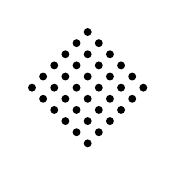
\begin{tikzpicture}[scale=1]
    \pgfmathsetmacro{\spacingX}{0.2}     % Pas du réseau en X
    \pgfmathsetmacro{\spacingY}{0.2}     % Pas du réseau en Y
    \pgfmathsetmacro{\circleRadius}{0.05} % Rayon des cercles
    \pgfmathsetmacro{\angleRot}{45}       % Angle de rotation
    \pgfmathsetmacro{\nCirclesX}{5}      % Nombre de cercles en X
    \pgfmathsetmacro{\nCirclesY}{5}      % Nombre de cercles en Y

    % Calcul du centre pour la rotation
    \pgfmathsetmacro{\xmin}{0}           % Coordonnée minimale en X
    \pgfmathsetmacro{\ymin}{0}           % Coordonnée minimale en Y
    \pgfmathsetmacro{\xmax}{\nCirclesX * \spacingX}
    \pgfmathsetmacro{\ymax}{\nCirclesY * \spacingY}
    \pgfmathsetmacro{\xcenter}{\xmax/2}
    \pgfmathsetmacro{\ycenter}{\ymax/2}

    % Appliquer la rotation
    \begin{scope}[rotate=\angleRot,shift={(\xcenter,\ycenter)}]
        \foreach \i in {0,...,\nCirclesX}{ % Boucle pour les colonnes
            \foreach \j in {0,...,\nCirclesY}{ % Boucle pour les lignes
                \pgfmathsetmacro{\x}{\xmin + \i * \spacingX}
                \pgfmathsetmacro{\y}{\ymin + \j * \spacingY}
                \fill[black] (\x-\xcenter, \y-\ycenter) circle (\circleRadius);
            }
        }
    \end{scope}
\end{tikzpicture}


